\documentclass[sigplan, anonymous, review]{acmart}

% Removes citation information below abstract
\settopmatter{printacmref=false}
% removes footnote with conference information in first column
\renewcommand\footnotetextcopyrightpermission[1]{}
%% removes running headers
\pagestyle{plain}

\usepackage[T1]{fontenc}
\usepackage{booktabs} % For formal tables
\usepackage{enumitem}
\usepackage{hyperref}
\usepackage{listings}
\usepackage{multirow}
\usepackage{subcaption}

\hypersetup{
  colorlinks=true,
  linkcolor=ACMRed,
  urlcolor=ACMBlue,
  citecolor=ACMRed,
}

\lstset{
  showspaces=false,
  showtabs=false,
  breaklines=true,
  showstringspaces=false,
  breakatwhitespace=true,
  escapeinside={(*@}{@*)},
  basicstyle=\scriptsize\ttfamily,
  columns=fullflexible,
  morekeywords={maybe_downsample, maybe_skip}
}

\setlength{\abovecaptionskip}{4pt}
\captionsetup{belowskip=12pt,aboveskip=4pt}

% Copyright
\setcopyright{none}
%\setcopyright{acmcopyright}
%\setcopyright{acmlicensed}
%\setcopyright{rightsretained}
%\setcopyright{usgov}
%\setcopyright{usgovmixed}
%\setcopyright{cagov}
%\setcopyright{cagovmixed}

%% Below is commented out for submission
% % DOI
% \acmDOI{10.475/123_4}

% % ISBN
% \acmISBN{123-4567-24-567/08/06}

% % Conference
% \acmConference[SOSP'17]{}{October 29--31, 2017}{Shanghai, China}
% \acmYear{2017}
% \copyrightyear{2017}
% \acmPrice{15.00}
% \acmBadgeL[http://ctuning.org/ae/ppopp2016.html]{ae-logo}

\begin{document}
\title{Resilient Wide-area Streaming Analytics \\
  with Automatic Profiling and Runtime Adaptation}

% The default list of authors is too long for headers}
\renewcommand{\shortauthors}{B. Zhang et al.}

\newcommand{\sysname}{AdaptiveStream}
\newcommand{\para}[1]{\smallskip\noindent\textbf{#1}}
\newcommand{\paraf}[1]{\smallskip\noindent\textbf{#1}}
\newcommand{\todo}[1]{{\color{ACMRed}\bf{TODO: #1}\normalfont}}

\def\Snospace~{\S{}}
\renewcommand*\sectionautorefname{\Snospace}
\renewcommand*\subsectionautorefname{\Snospace}
\renewcommand*\subsubsectionautorefname{\Snospace}
\renewcommand*{\equationautorefname}{Eq.}
\renewcommand*{\figureautorefname}{Fig.}

%%% Local Variables:
%%% mode: latex
%%% TeX-master: "sosp17"
%%% End:


\begin{abstract}
  In the wide area, the emerging class of streaming analytics faces the
  challenge of scarce and variable network bandwidth. Existing approaches that
  adapt to network changes are either application-specific solutions or they
  require extensive developers' effort.

  In this paper, we present \sysname{}, a stream processing system that adapts
  application execution with minimal developer efforts.
\end{abstract}

% The code below should be generated by the tool at
% http://dl.acm.org/ccs.cfm
% Please copy and paste the code instead of the example below.
%
\begin{CCSXML}
<ccs2012>
  <concept>
    <concept_id>10010520.10010521.10010537</concept_id>
    <concept_desc>Computer systems organization~Distributed architectures</concept_desc>
    <concept_significance>300</concept_significance>
  </concept>
  <concept>
    <concept_id>10010520.10010570.10010574</concept_id>
    <concept_desc>Computer systems organization~Real-time system architecture</concept_desc>
    <concept_significance>300</concept_significance>
  </concept>
  <concept>
    <concept_id>10002951.10003227.10003251.10003255</concept_id>
    <concept_desc>Information systems~Multimedia streaming</concept_desc>
    <concept_significance>300</concept_significance>
  </concept>
  <concept>
    <concept_id>10002951.10003227.10010926</concept_id>
    <concept_desc>Information systems~Computing platforms</concept_desc>
    <concept_significance>300</concept_significance>
  </concept>
</ccs2012>
\end{CCSXML}

\ccsdesc[300]{Computer systems organization~Distributed architectures}
\ccsdesc[300]{Computer systems organization~Real-time system architecture}
\ccsdesc[300]{Information systems~Multimedia streaming}
\ccsdesc[300]{Information systems~Computing platforms}

\keywords{adaptation, learning, stream processing}

%% Below is the code to create the teaser
% \begin{teaserfigure}
%   \includegraphics[width=\textwidth]{sampleteaser}
%   \caption{This is a teaser}
%   \label{fig:teaser}
% \end{teaserfigure}

\maketitle

\section{Introduction}

%% Background
Wide-area streaming analytics are becoming pervasive, especially with the
emerging class of Internet of Things (IoT) applications.  Large cities such as
London and Beijing have deployed millions of cameras for surveillance and
traffic control~\cite{skynet, london.surveillance}. Buildings are increasingly
equipped with a wide variety of sensors to improve energy efficiency and
occupant comfort~\cite{krioukov2012building}. Geo-distributed infrastructure,
such as content delivery networks (CDNs), analyzes requests from machine logs
over the globe~\cite{mukerjee2015practical}. These applications need to
transport, distill and process streams of data across the wide area in real
time.

Although existing stream processing systems, such as
Storm~\cite{toshniwal2014storm}, Spark Streaming~\cite{zaharia2013discretized},
and VideoStorm~\cite{zhang2017live}, can handle large streams of data, they are
designed to work within a single cluster, where the network is not the
bottleneck.  In contrast, the wide area network (WAN) has limited
bandwidth~\cite{hsieh17gaia, vulimiri2015global}. Moreover, WAN bandwidth growth
has been decelerating for many years~\cite{global2016telegeography} while
traffic demands are growing at a staggering rate~\cite{index2013zettabyte}.

Limited WAN bandwidth makes it neither practical nor efficient to back-haul all
data to a central location.  Recent research on WAN-aware systems promotes
pushing computations towards the edge~\cite{pu2015low, rabkin2014aggregation,
  satyanarayanan2009case}. However, communication is not entirely avoidable:
$(i)$ some analytical jobs require joining or aggregating data from multiple
geo-distributed sites~\cite{pu2015low, viswanathan2016clarinet}; $(ii)$ the edge
benefits substantially from central computing resources such as GPUs and
TPUs~\cite{abadi2016tensorflow} in the cloud; and $(iii)$ end-devices such as
cameras and mobile devices suffer from limited bandwidth in last-hop wireless
links when running processing on nearby edge
infrastructure~\cite{abari2017enabling, zhang2015design}.

% could improve efficiency (such as GDA pushes queries out; cloudlet
% etc). However, we still need data transmission for cloud off-loading or
% aggregation purpose.

When facing insufficient bandwidth, application developers need to make a
decision within the design space of data fidelity versus freshness
(\autoref{fig:intro}).

\begin{figure}
  \centering
  \includegraphics[width=0.8\columnwidth]{figures/figure1.pdf}
  \caption{The trade-off space between data freshness and fidelity when facing
    insufficient bandwidth (details in \autoref{sec:runtime-adaptation}).}
  \label{fig:intro}
  \vspace{-1em}
\end{figure}

Applications using existing protocols without adaptation result in extreme
design points. Streaming over TCP ensures a reliable delivery but backlogged
data increases latency. On the other hand, streaming over UDP minimizes latency
by sending packets as fast as possible, but uncontrolled loss devastates
application accuracy.

Degradation, as demonstrated by JetStream~\cite{rabkin2014aggregation}, allows
developers to trade data fidelity for freshness. While it's easy to write
policies for simple operations, such as sampling, in general, accurate policies
will require extensive expertise and considerable efforts. In practice,
developers write policies based on some set of heuristics rather than
quantitative measurements. These inaccurate manual degradation policies lead to
sub-optimal performance for both freshness and fidelity.

Furthermore, application-specific optimizations do not generalize. A fine-tuned
adaptation algorithm for one application will work poorly for another
application, if performance metrics or data distributions change.  For example,
video streaming focuses on quality of experience
(QoE)~\cite{michalos2012dynamic, pantos2016http, yin2015control}. Because humans
favor smoothness over image quality, video streaming systems maintain a high
frame rate, e.g.\,\(25~\text{FPS}\), and reduce image resolutions under
bandwidth limit.  Adaptation by reducing resolutions is a poor match for
analytic jobs that rely on image details.

To achieve low latency and high accuracy simultaneously with minimal developer
effort, we design and implement \sysname{}, a stream processing system for the
wide area. The key idea is to build an accurate and precise performance model
instead of relying on manual or application-specific policies. \sysname{}'s
solution is three-fold: easy-to-use APIs, automatic profiling, and a low-latency
runtime.

\sysname{} augments existing stream processing operators with a new \maybe{}
operator. Its basic form takes a list of values as a knob and a function that
degrades the input stream. The knob specifies the degradation level that affects
data size and data fidelity. We extend the basic form with a library of
specialized operators for common data types, such as \texttt{maybe\_downsample}
for images. Our APIs are simple, composable and extensible. Developers do not
need to be an expert in the application domain as the knobs tolerate approximate
specifications. Multiple operators form a configuration that affects the
adaptation jointly. Arbitrary functions and external libraries can be embedded
with our operators.

\sysname{} then uses a data-driven approach to automatically build application
performance profiles with minimal developer effort. The profiles accurately
capture the relationship between application accuracy and bandwidth consumption
under different combinations of data degradation operations. We use an offline
process to bootstrap our system with developer-supplied training data, and
continuously refine the profile online to handle model drifts. We exploit
parallelism and sampling-based profiling to efficiently explore the
configuration space and learn a Pareto-optimal adaptation strategy.

At runtime, \sysname{} achieves low latency by matching data rate to available
bandwidth, and high accuracy by using Pareto-optimal configurations from the
profile. Upon network congestion, our rate adaptation algorithm increases the
degradation level to reduce data rate, such that no persistent queue builds
up. To recover, it progressively decreases the degradation level after probing
for more available bandwidth. The runtime also provides additional options for
developers to control application behaviors, e.g., limiting the maximum allowed
WAN bandwidth. For multiple applications, the profiles allow bandwidth
allocation among competing tasks for utility fairness.

To evaluate \sysname{}, we've built three streaming applications: augmented
reality (AR), pedestrian detection (PD), and distributed Top-K analysis (TK). We
use real-world data to profile these applications and evaluate their runtime
performance on a geo-distributed public cloud. Our contributions and evaluation
results are as follows.

\begin{itemize}[leftmargin=*, topsep=2pt, itemsep=2pt]

\item We propose \maybe{} operators to incorporate adaptation with existing
  stream processing models. Our programming abstraction is simple, composable
  and extensible.

\item We show that \sysname{}'s data-driven approach generates an accurate and
  precise profile for each application. Parallelism and sampling techniques
  can speed up the profiling substantially, up to 29$\times$ and 9$\times$\@.

\item Using runtime experiments on geo-distributed EC2 nodes, \sysname{}
  achieves low latency and high accuracy simultaneously for all
  applications---sub-second latency and 2\% accuracy drop for video analytics,
  4-second latency and 1\% accuracy drop for TK\@.

\end{itemize}

%%% Local Variables:
%%% mode: latex
%%% TeX-master: "awstream"
%%% End:

%% LocalWords: VideoStorm, analytics, CDN, IoT

\section{Motivation}
\label{sec:background-motivation}

In this section, we make the case for an adaptive stream processing system in
the wide area by examining the gap between application demands and the existing
infrastructure. We start with a few streaming applications.

\para{Video Surveillance:} We envisage a city-wide monitoring system that
aggregates camera feeds (both stationary ground cameras and moving aerial
vehicles) and analyzes video streams in real-time for surveillance, anomaly
detection or business intelligence~\cite{oh2011large}. While traditionally human
labors are involved in analyzing abnormal activities, recent advances in
computer vision and deep learning has dramatically increased the accuracy for
automatic analysis of visual scenes, such as pedestrian
detection~\cite{dollar2012pedestrian}, vehicle tracking~\cite{coifman1998real},
or facial recognition to locate people of interest~\cite{parkhi2015deep,
  Lu:2015:SHF:2888116.2888245}. \todo{Add concrete numbers to argue for the data
  volume.}

\para{IoT Sensors:} While traditional environmental sensors are
slow~\cite{atzori2010internet}, we are seeing an increasing trend with
high-frequency, high-precision sensors being deployed. For example, uPMU
monitoring system for the electrical grid consists of a network of 1000 devices;
each produces 12 streams of 120 Hz high-precision values accurate to 100
ns. This amounts to 1.4 million points per second that requires specialized
timeseries database~\cite{andersen2016btrdb}.

\para{Log Analysis:} Large organizations today are managing 10--100s of
datacenters (DCs) and edge clusters worldwide~\cite{calder2013mapping}. While
most log analysis today runs in a batch mode and on a daily basis, there is
trend in analyzing logs in real-time for quicker optimization \todo{cite RISE
  reference?}. For example, a content distribution network (CDN) can improve the
overall efficiency by optimizing data placement if the access logs can be
processed in real-time.

\vspace{0.5em}

We consider the practical issues with deploying these applications. While they
challenge the data storage and processing system, the cloud can handle it well.
The real challenge lies in the communication. Data generated from the edge, not
a lot WAN bandwidth; also with cost. And worse, the bandwidth is also not
guaranteed. We will demonstrate with measurement.

\subsection{Wide-Area Bandwidth Characteristics}
\label{sec:making-case-adapt}

\begin{figure}
  \centering
  \includegraphics[width=.95\linewidth]{figures/europe-to-us-west.pdf}
  \caption{Bandwidth measurement between Amazon EC2 sites (from Ireland to
    California).}
  \label{fig:bw}
\end{figure}

To understand the bandwidth characteristics in the wide-area, we conducted a
simple measurement using Amazon EC2. We use iPerf~\cite{iperf} to measure the
pair-wise bandwidth between four geo-distributed sites throughout the day. We
observed large variance in the measured bandwidth and one such pair is shown in
\autoref{fig:bw}. Regardless of the number of flows\footnote{EC2 has a per-flow
  and per-VM rate limiting~\cite{zhang2016guaranteeing}.}, these exist occasions
when the available bandwidth is almost halved. We believe the backhaul links
between EC2 sites are better (if not at least representative) in comparison to
the general wide-area links. The varying nature poses real challegen to the
realization and successful deployment of wide-area streaming applications.

\subsection{Bandwidth-Accuracy Trade-off}
\label{sec:bat}

% Existing stream processing systems in the wide area often directly use TCP as
% their transport. TCP works remarkably well estimating the available bandwidth
% and minizing flow completion time. Although TCP adapts the congestion window in
% dynamically based on the feedback from the
% receiver~\cite{jacobson1988congestion}, being application agnostic, TCP delivers
% whatever the application wants to send; and in the case of limited network
% capacity, TCP creates backlogged data, causing significant delay.

% For applications where TCP's retransmission is not unnessary, UDP is often
% chosen. Many multimedia applications such as Internet
% telephony~\cite{baset2004analysis}. Live IP cameras streaming with RTMP. Or
% sensor data over OSC~\cite{wright1997open}, a protocol based on UDP. UDP's
% packet loss can be detrimental in the deteriorate situations.

% The issue with these protocol is that they are designed to be generally
% applicable to many applications without intervening the application execution.
% Often developers of individual applications need to tune the transport to fit
% their needs~\cite{tierney2001tcp} or deal with the insufficient bandwidth case.

The edge infrastructure is capable of pre-processing the data before the
communication. Data degradation. Such as frame-diff based video encoding
scheme. In the case of the top-K application, we first generate windowed local
counts. In our dataset, we see 100x data size reduction. While effective, these
transformations are often not sufficient. In the case of top-k, there is a long
tail. In the case of images/video, quantizing individual pixels will often give
more space.

They help reduce the resource demand but they typically also lower the output
quality. \autoref{fig:log-trade-off} shows how the image resolution affects
application accuracy.

In some verticle domain, such as video encoding, adaptive scheme
exists. However, there is no general solution and these solutions are not
generally applicable to all applications. Most video encoding techniques will
adjust the quantizer to tune the encoding size and quality; while often
preserving the frame rate as these videos are for human consumption. A smooth
video provides a better quality of experience than higher resolution but
intermitten images.

We presented empirical results with grouped, windowed aggregation on PlanetLab
using Akamai log data, and highlighted the complexity of tradeoffs that we show
are driven by several factors such as query, data, and resource
characteristics. local aggregation and global
aggregation.~\cite{heintz2015towards}

This motivates us to design an application-aware rate-adapting stream processing
framework for the wide area; primarily exploring the design space of
degradation.

For these applications, there is a trade-off between the bandwidth and accuracy.
Exploring the design space that allows explicit trading accuracy for resource
constrained cases is the main goal of this paper.

\begin{figure}
  \centering
  \begin{subfigure}{.48\columnwidth}
    \centering
    \includegraphics[width=.95\linewidth]{figures/motiv-resolution.pdf}
    \label{fig:log-bw}
  \end{subfigure}
  \begin{subfigure}{.48\columnwidth}
    \centering
    \includegraphics[width=.95\linewidth]{figures/motiv-framerate.pdf}
    \label{fig:log-acc}
  \end{subfigure}
  \caption{The trade-off between required bandwidth and the accuracy.}
  \label{fig:log-trade-off}
\end{figure}

%%% Local Variables:
%%% mode: latex
%%% TeX-master: "sigcomm2017"
%%% End:

\section{\sysname{}}
\label{sec:system}

In contrast to existing approaches that require developers to specify the
concrete policies, \sysname{} uses a special operator \texttt{maybe} to express
structured adaptation. The specifications are hints on potential operations
without exact quantifications. \sysname{} then automatically learns concrete
degradation strategies (the profile) using profiling data (either offline or
online) and controls the application execution at runtime. The profiles also
have additional benefits such as coordination among competing streaming
flows. \autoref{fig:overview} provides an overview of the systems (in three
stages) and we describe each stage in turn.

\begin{figure}
  \centering
  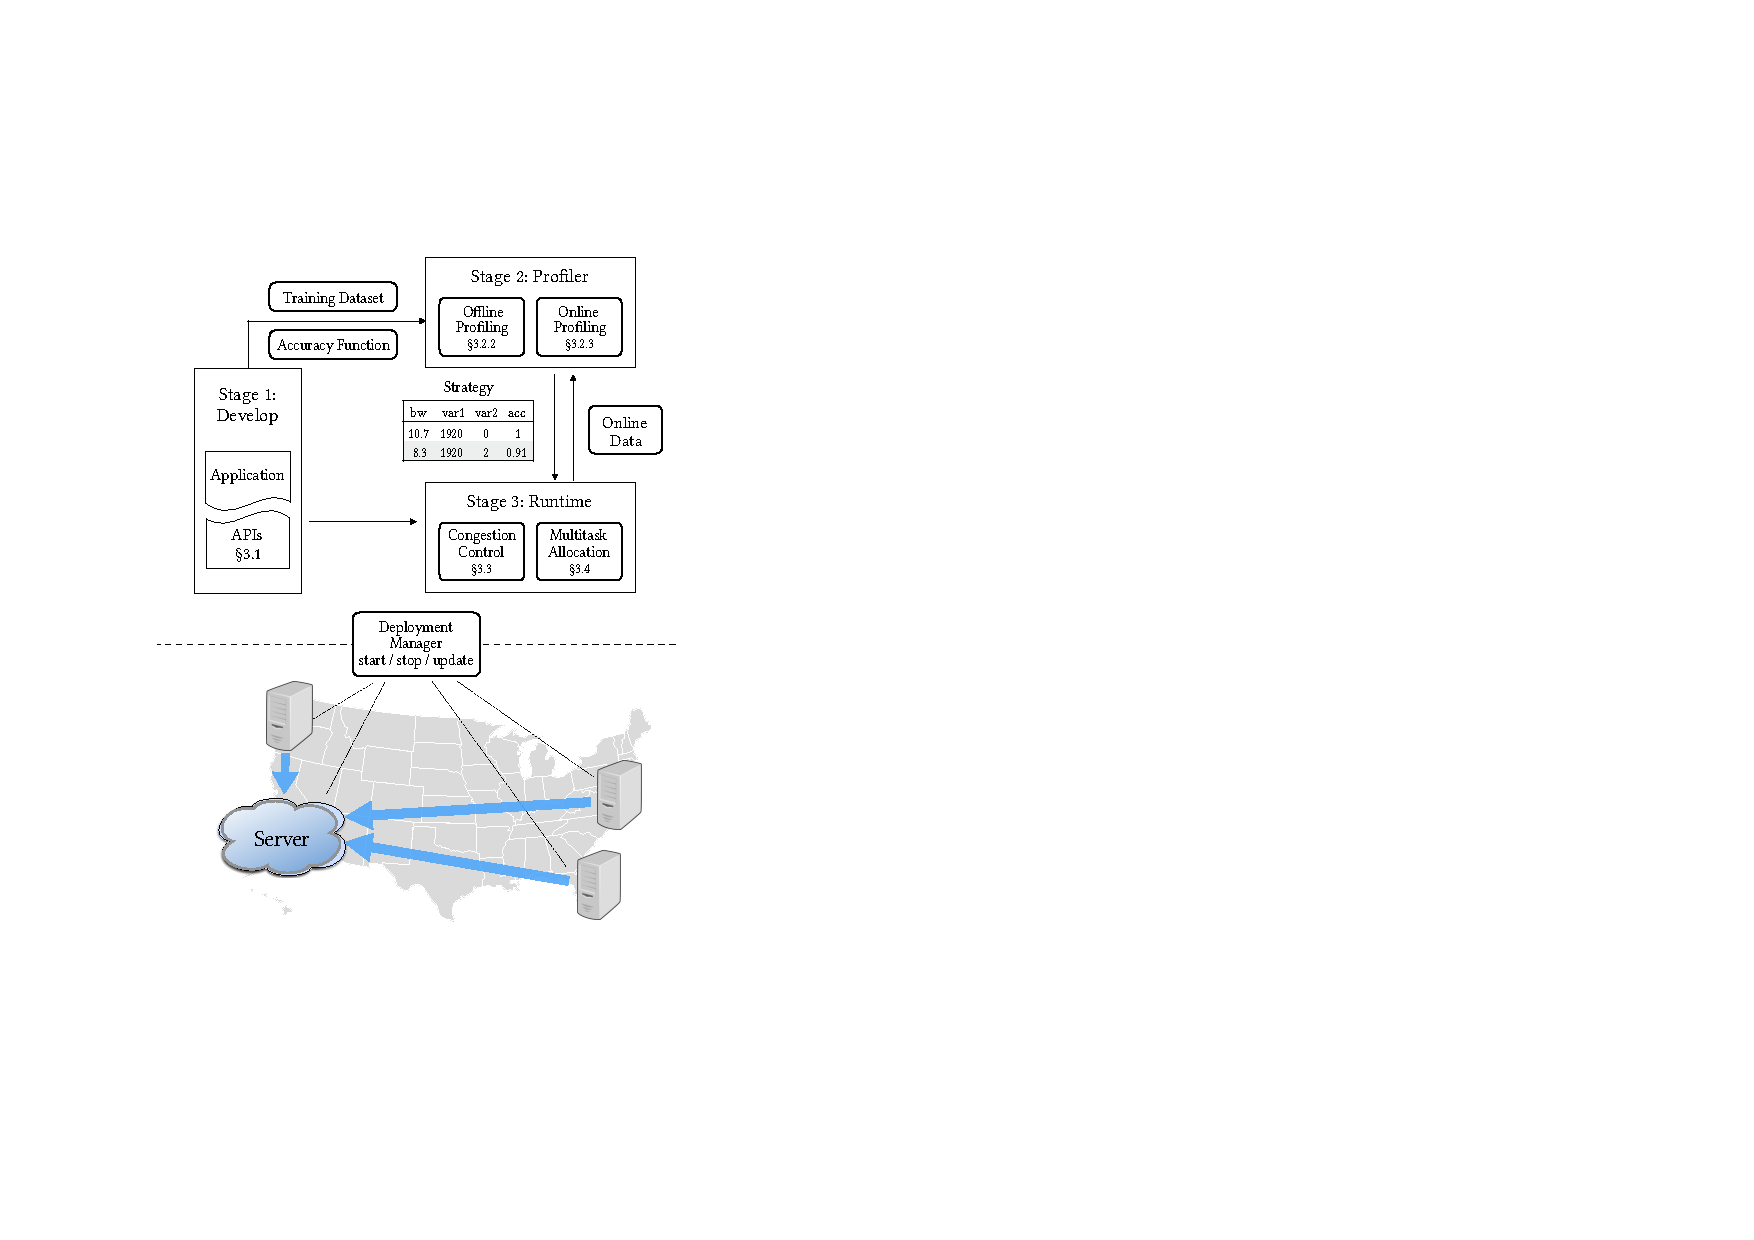
\includegraphics[width=.9\linewidth]{figures/system.pdf}
  \caption{High-level overview of \sysname{}.}
  \label{fig:overview}
\end{figure}

\begin{table*}
  \small
  \centering
  \begin{tabular}{ c r l }
    \toprule
    \multirow{5}{*}{Normal Operators}
    & \textit{map} (f: I $\Rightarrow$ O) & Stream<I> $\Rightarrow$ Stream<O> \\
    & \textit{skip} (i: Integer) & Stream<I> $\Rightarrow$
                                   Stream<I> \\
    & \textit{sliding\_window} (count: Integer, f: Vec<I> $\Rightarrow$ O) & Stream<I> $\Rightarrow$
                                                                            Stream<O> \\
    % & \textit{tumbling\_window} (count: Integer, f: Vec<I> $\Rightarrow$ O) & Stream<I> $\Rightarrow$
    %                                                                          Stream<O> \\
    & \textit{timed\_window} (time: Duration, f: Vec<I> $\Rightarrow$ O) & Stream<I> $\Rightarrow$
                                                                          Stream<O> \\
    & ... & ... \\
    \midrule
    \multirow{5}{*}{Degradation Operators}
    & \textit{maybe} (knobs: Vec<T>, f:  (T, I) $\Rightarrow$ I) & Stream<I> $\Rightarrow$
                                                                 Stream<I> \\
    & \textit{maybe\_skip} (knobs: Vec<Integer>) & Stream<I> $\Rightarrow$ Stream<I> \\
    & \textit{maybe\_head} (knobs: Vec<Integer>) & Stream<Vec<I>{}> $\Rightarrow$
                                                   Stream<Vec<I>{}> \\
    & \textit{maybe\_downsample} (knobs: Vec<(Integer, Interger)>) & Stream<Image> $\Rightarrow$ Stream<Image> \\
    & ... & ... \\
    \bottomrule
  \end{tabular}
  \caption{Stream processing operators in \sysname{}. \texttt{Vec<T>} represents
    a list of elements with type \texttt{T}.}
  \label{tab:operators}
\end{table*}

\subsection{APIs for Structured Adaptation}
\label{sec:struct-adapt}

%% Introduce graphs of operators model
The majority of stream processing applications today are constructed as a
directed graph of operators~\cite{toshniwal2014storm, zaharia2013discretized},
where each operator transforms input streams into new streams. \sysname{}
borrows the same computation model. We list some example operators, such as
\texttt{map} and \texttt{skip}, in \autoref{tab:operators}.

Along with normal operators, \sysname{} integrates special \maybe{} operators
that degrades the data quality, yielding potential bandwidth savings. Our design
has the following goals: (i) to free developers from specifying exact rules, the
API should tolerate approximate specifications; (ii) to allow combining multiple
dimensions, the API should be modular: each operator is a unit and developer can
chain multiple operators; (iii) to support flexible integration with arbitrary
degradation functions, the API should take user-defined functions
(UDFs). Therefore, our API is,
\vspace{-2pt}
\begin{lstlisting}
        maybe(knobs: Vec<T>, f: (T, I) => I)
\end{lstlisting}

We illustrate the usage of \texttt{maybe} operator with an example that
quantizes a stream of integers in Rust:

\vspace{-2pt}
\begin{lstlisting}
    let quantized_stream = vec![1, 2, 3, 4].into_stream()
        .maybe(vec![2, 4], |k, p| p.wrapping_div(k));
        .collect();
\end{lstlisting}

The snippet creates a stream of integers, chains a degradation operation and
collects the execution result. In this example, the knob is [2, 4], and the
degradation function performs a wrapping (modular) division where the divisor is
the chosen knob. The knob value modifies the quantization level, affecting the
output: [1, 2, 3, 4] (no degradation), [0, 1, 1, 2] (k=2), or [0, 0, 0, 1]
(k=4). If the stream is subsequently encoded---for example, run-length encoding
as in JPEG~\cite{wallace1992jpeg}---for transmission, the bandwidth consumption
will change according to the level of degradation.

Based on the \texttt{maybe} primitive, one can implement wrappers of degradation
operations for common data types. For instance, \texttt{maybe\_head} will
optionally takes the top values of the \textit{list}; and
\texttt{maybe\_downsample} can adjust the \textit{image} resolution to a
configured target. \sysname{} provides a few such operations as libraries for
developers (\autoref{tab:operators}).

With our APIs, the example mentioned in \autoref{sec:making-case-sys-approach}
can now be implemented as follows:

\vspace{-2pt}
\begin{lstlisting}[caption={Video Processing Example}, label={lst:ex}]
   let app = Camera::new((1920, 1080, 30))
      .maybe_downsample(vec![(1600, 900), (1280, 720)])
      .maybe_skip(vec![2, 5])
      .map(|frame| frame.show())
      .compose();
\end{lstlisting}

This snippet first instantiates a \texttt{Camera} source, which produces
\texttt{Stream<Image>} with 1920x1080 resolution and 30 FPS. Two degradation
operations follow the source: one that downsamples image to either 1600x900 or
1280x720 resolution; one that skips frames with a parameter of 2 or 5, resulting
in 30/(2+1)=10 FPS or 30/(5+1)= 6 FPS. In this example, degraded images are
shown on the display, while in practice, further processing, such as encoding
and transmission, operators can be chained.

Structured adaptation not only simplifies the specifications of degradation, the
structure also facilitates learning an accurate profile
(\autoref{sec:automatic-profiling}) and reacting at runtime
(\autoref{sec:runtime}).

%%% Local Variables:
%%% mode: latex
%%% TeX-master: "sosp17"
%%% End:

\subsection{Automatic Profiling}
\label{sec:automatic-profiling}

The goal of the profiling is to learn how different levels of degradation
affects the bandwidth demand and application accuracy. By exploring this
trade-off space, \sysname{} generates a Pareto-optimal \textit{profile} for each
application. We formulate the profiling and discuss the designs for offline and
online profiling.

\subsubsection{Profiling Formalism}
\label{sec:formalize-profiling}

Suppose in a stream processing application that $n$ \maybe{} operators are
used. Each introduces a knob $k_i$. We assume these operators are independent
from each other; their combination forms a \textit{configuration}
$c = [k_{1}, k_{2}, ... k_{n}]$. The set of all possible configurations
$\mathbb{C}$ is the space that our profiling system needs to explore. For each
configuration $c$, there are two mappings that our system needs to explore: a
mapping from $c$ to its bandwidth requirement $B(c)$ and its accuracy measure
$A(c)$. \autoref{tab:notations} summarizes the symbols used in this paper.

The Pareto-optimal set $\mathbb{P}$ is then defined (\autoref{eq:pareto}): for
all $c \in \mathbb{P}$, there is no alternative configuration $c'$ that requires
less bandwidth while giving a higher accuracy.

{\small
\begin{equation}
  \mathbb{P} = \{ c \in \mathbb{C} : \{ c' \in \mathbb{C}: B(c') < B(c),
  A(c') > A(c) \} = \varnothing\}
  \label{eq:pareto}
\end{equation}
}%

\begin{table}
  \small
  \centering
  \begin{tabular}{r l}
    \toprule
    \textbf{Symbol} & \textbf{Description} \\
    \midrule
    $n$ & number of degradation operations \\
    $k_i$ & the \textit{i}-th degradation knob \\
    $c = [k_{1}, k_{2}, ... k_{n}]$ & one specific configuration \\
    $\mathbb{C}$ & the set of all configurations \\
    \midrule
    $B(c)$ & bandwidth requirement for $c$ \\
    $A(c)$ & accuracy measure for $c$ \\
    $\mathbb{P}$ & Pareto efficienct set \\
    \bottomrule
  \end{tabular}
  \caption{Notations used in profiling (keep?).}
  \label{tab:notations}
\end{table}

Since there is often no closed form relation for $B(c)$ and $A(c)$, our system
takes a data-driven approach: with a representative training dataset and an
application-specific utility function, our system evaluates each configuration
for its bandwidth and accuracy. The accuracy can either be measured against the
groundtruth; or in the case when labelled dataset is not available, \sysname{}
uses the results when all degradations are turned off as the reference. We will
discuss concrete knobs, configurations, $B(c)$ and $A(c)$ when we present the
example applications in \autoref{sec:build-appl}.

\subsubsection{Offline Profiling}
\label{sec:offline-profiling}

The offline profiling requires an exhaustive search. Developers using \sysname{}
will first perform an offline profiling that generates the Pareto-optimal
profile by supplying training dataset and application accuracy function. Because
our APIs are general, there is no restriction in the values or functions
provided for \maybe{}. Without \textit{a prior}, any configuration is possible
to be inside the optimal profile.

The exhaustive search is expensive. Therefore, the offline profiling requires to
explore the entire parameter space, which is a combinatorial space of all
knobs. For \textit{offline}, the time required is acceptable.

We note that parallelism is usable for profiling. Except for the groundtruth (or
reference label), two different configurations have no dependence over each
other. Making the profiling an embarrassingly parallel task.

cite ernest experiment design.

\subsubsection{Online Profiling}
\label{sec:online-profiling}

The offline profile is susceptible to ``model drift''. When the required
bandwidth is underestimated, data will be queued at the sender and application
latency will increase. When the accuracy is incorrectly measured, the actual
application performance will be suboptimal. The drift needs to be corrected
online. There are two particular challenges for online profiling.

The first is the lack of groundtruth data or reference data. During the online
execution, it's often infeasible to get labelled data as the groundtruth. For
example, image labelling is known to be labor intensive and time
consuming~\cite{russell2008labelme}. In addition, the original un-degraded data
need to be transmitted from the sender. \sysname{} addresses labelling by using
the un-degraded data as the reference and allocate additional bandwidth for
backhaulling portions of the un-degraded data. While the additional bandwidth
seems a waste, in our design, during the runtime's probing phase, the original
data can enjoy a free ride. Details of the probing is in \autoref{sec:runtime}.

The second challenge is how to profile efficiently. We use the offline profiling
information as a prior to speed-up the online profiler. Specficially, we employ
two techniques: degradation-aware parallelization and partial profiling.

\para{Degradation-aware parallelization:} The profiling tasks of exploring all
configurations are easily parallelizable. Normal job schedulers don't assume the
knowledge of estimated task completion time, therefore the parallel execution
suffers from sub-optimal assignments. Aided with the offline profiling
statistics (the time it requires to profile a particular configuration), we can
schedule the online profiling tasks with a longest first scheduling that
minimizes the makespan.

\para{Partial profiling:} In time domain, the profiling could use a smaller
chunk of data to approximate the best strategy. Besides, we can profiling a
subset of the total configurations and measures its difference from the current
profile. If the difference exceeds a certain threshold, it triggers a full
profiling.

%%% Local Variables:
%%% mode: latex
%%% TeX-master: "sosp17"
%%% End:

\subsection{Runtime Adaptation}
\label{sec:runtime}

\begin{figure}
  \centering
  \resizebox{\columnwidth}{!}{
    \begin{tikzpicture}
  %
  % Define basic styles
  %
  % Node
  \tikzstyle{module} = [draw, very thick, rounded corners,
  fill=white, minimum height=2.5em, inner sep=0.5em,
  rectangle, font={\bfseries}, align=center]
  \tikzstyle{cmodule} = [module, fill=black!20]

  % Edge
  \tikzstyle{stateEdgePortion} = [black, thick];
  \tikzstyle{dataEdge} = [stateEdgePortion, ->];
  \tikzstyle{controlEdgePartial} = [stateEdgePortion, dashed];
  \tikzstyle{controlEdge} = [controlEdgePartial, ->];
  \tikzstyle{controlDoubleEdge} = [controlEdgePartial, <->];
  \tikzstyle{edgeLabel} = [pos=0.5, text centered, font={\itshape}];

  \node[name=client, draw, very thick, fill=white,
  double copy shadow={shadow xshift=2pt, shadow yshift=-2pt, fill=white, draw},
  text height=13em, text width=31.5em] {};

  \node[name=server, draw, very thick, fill=white, draw,
  right=of client.north east, anchor=north west, xshift=1em,
  text height=7em, text width=12.5em] {};

  \node[module, name=source, below right=of client.north west,
  xshift=-1.5em, yshift=1.5em] {Source};
  \node[module, name=transform, right of=source, xshift=3.5em] {Transform};
  \node[cmodule, name=degrade, right of=transform, xshift=3.7em] {Degrade};
  \node[cmodule, name=queue, right of=degrade, xshift=3em] {Queue};
  \node[cmodule, name=socket, right of=queue, xshift=3em, text width=3em] {Socket};
  \node[cmodule, name=receiver, right of=socket, xshift=7em] {Receiver};
  \node[module, name=analytics, right of=receiver, xshift=3em] {Analytics};

  \node[cmodule, name=cc, at=($(queue)!0.5!(socket)$), yshift=-6em]
  {Congestion\\Controller};

  \draw ($(source.east)$) edge[dataEdge] ($(transform.west)$);
  \draw ($(transform.east)$) edge[dataEdge] ($(degrade.west)$);
  \draw ($(degrade.east)$) edge[dataEdge] ($(queue.west)$);
  \draw ($(queue.east)$) edge[dataEdge] ($(socket.west)$);
  \draw ($(socket.east)$) edge[dataEdge] node[edgeLabel, yshift=0.6em] {data}
  ($(receiver.west)$);
  \draw ($(receiver.east)$) edge[dataEdge] ($(analytics.west)$);

  %% Control path
  \draw let
  \p1 = ($(cc.center)$), \p2 = ($(degrade.center)$)
  in ($(cc.west)$) edge[controlEdgePartial] (\x2, \y1)
  (\x2, \y1) edge[controlEdge] ($(degrade.south)$);

  \draw let
  \p1 = ($(queue.south)$), \p2 = ($(cc.north)$)
  in ($(\x1, \y1) + (1em,0)$) edge[controlEdge] ($(\x1, \y2) + (1em,0)$);

  \draw let
  \p1 = ($(socket.south)$), \p2 = ($(cc.north)$)
  in ($(\x1, \y1) + (-1em,0)$) edge[controlDoubleEdge] ($(\x1, \y2) + (-1em,0)$);

  \node[name=clientlabel, above right=of client.south west, xshift=-2em, yshift=-2em] {Edge (Client)};
  \node[name=clientlabel, above left=of server.south east, xshift=2em, yshift=-2em] {Server};

  %%
  %% Legend
  %%
  \node[name=datalegend, below=1.5em of server.south west, xshift=2em]
  {\small Data Plane};
  \draw ($(datalegend.west) + (-2em, 0)$) edge[dataEdge]
  ($(datalegend.west) + (-0.5em, 0)$);

  \node[name=controllegend, below=2.5em of datalegend.west, anchor=west]
  {\small Control Plane};
  \draw ($(controllegend.west) + (-2em, 0)$) edge[controlEdge]
  ($(controllegend.west) + (-0.5em, 0)$);

  \node[name=applegend, right=3em of datalegend.east]
  {\small Application Logic};
  \node[module, name=applegendbox, left=0.1em of applegend, text width=0.3em,
  minimum height=0em] {};

  \node[name=syslegend, below=2.5em of applegend.west, anchor=west]
  {\small Runtime};
  \node[cmodule, name=syslegendbox, left=0.1em of syslegend, text width=0.3em,
  minimum size=0em] {};

\end{tikzpicture}

%%% Local Variables:
%%% mode: latex
%%% TeX-master: "sosp17"
%%% End:

  }
  % \includegraphics[width=\linewidth]{figures/runtime-adaptation.pdf}
  \caption{Runtime adaptation system architecture. The grey components are what
    \sysname{} provides.}
  \label{fig:runtime}
\end{figure}

At runtime, the user program is automatically converted to a client half and
server half; and \sysname{} abstracts the communication as well as rate
adaptation (\autoref{fig:runtime}).

The data source with degradation is a module that supports \texttt{update}
function. To handle insufficient bandwidth, an object-level queue bridges data
generation (source) and the network IO. Followed by the queue is a socket module
that abstracts the network communication. It transmits data as fast as possible
and also supports traffic probing. The growth of the queue indicates congestions
and will trigger the congestion controller. The socket module estimates actual
available bandwidth. To avoid spikes in the bandwidth measurement, exponential
smoothing is employed.

At the core of our rate adjustment is a congestion control algorithms assisted
with stream data generation rate (\autoref{fig:cc}).

\para{Startup behavior:} When the application starts up, it performs its first
(and most rapid) rate increase. On each \texttt{Q.NoQueue} received, it
decreases the level of degradation, hence an increase of the data rate.

\para{Reacting to congestion:} When congestion is detected by an increase of the
queued item, TCP's send rate is used as an approximation of the bottleneck
bandwidth of the current connection. \sysname{} then adjusts the level of
degradation such that the expected data rate is below the estimated bandwidth
(often with a factor to allow the queue draining). After the queue is drained
and there is no queued item for a configurable period, it fires
\texttt{Q.NoQueue} event to the congestion controller, which then enters into
the \texttt{Steady} state.

\para{Steady state:} The steady state is the ideal state that the streaming
application should stay in. If currently the application is operating at the
maximum rate, then there is no need to probe. However, we might be in steady
state with degradation, in this case, we need to probe to test if there is more
bandwidth. Enter probe state.

\para{Probe for available bandwidth:} In contrast to BBR that adjusts the pace
of transmission, our probe is to send dummy traffic. If the application is
configured to run online profiling, then the probe traffic is the raw data.

% \begin{figure}
%   \centering
%   \resizebox{\columnwidth}{!}{
%     \begin{tikzpicture}[
  state/.style = { draw, very thick, fill=white, rounded corners=1em,
    minimum height=3em, minimum width=7em, node distance=7em, font={\bfseries},
    align=center },
  edge portion/.style = { black, thick },
  transition/.style = { edge portion, -> },
  algorithm/.style = { draw, thin, fill=white },
  ]

  \node [state] (startup) {
    STARTUP };
  \node [state] (congestion) [right=of startup] {CONGESTION};
  \draw [transition] (startup) -- (congestion)
  node [midway, auto] {Q.Congestion};

  \node [state] (steady) [below=of congestion] {STEADY};

  \draw [transition] ($(congestion.south west)!0.4!(congestion.south east)$)
  to node[midway, sloped, below] {Q.NoQueue}
  ($(steady.north west)!0.4!(steady.north east)$);

  \draw [transition] ($(steady.north west)!0.6!(steady.north east)$)
  to node[midway, sloped, below] {Q.Congestion}
  ($(congestion.south west)!0.6!(congestion.south east)$);

  \node [state] (probe) [left=of steady] {PROBE};

  \draw [transition] ($(steady.south west)!0.6!(steady.north west)$)
  -- ($(probe.south east)!0.6!(probe.north east)$)
  node[midway, auto, swap] {Q.Probe};

  \draw [transition, <-] ($(steady.south west)!0.4!(steady.north west)$)
  -- ($(probe.south east)!0.4!(probe.north east)$)
  node[midway, auto, align=left] {Q.Congestion | \\ IO.ProbeDone};

\end{tikzpicture}


%%% Local Variables:
%%% mode: latex
%%% TeX-master: "sosp17"
%%% End:

%   }
%   \caption{Congestion Control Algorithm}
%   \label{fig:cc}
% \end{figure}

\begin{figure}
  \centering
  \includegraphics[width=\columnwidth]{figures/cc.pdf}
  \caption{Congestion Control Algorithm}
  \label{fig:cc}
\end{figure}

%%% Local Variables:
%%% mode: latex
%%% TeX-master: "sosp17"
%%% End:

\subsection{Multitask Adaptation}
\label{sec:multitask-adaptation}

Briefly discuss the issues without coordination.

\newpage

%%% Local Variables:
%%% mode: latex
%%% TeX-master: "sosp17"
%%% End:


%%% Local Variables:
%%% mode: latex
%%% TeX-master: "sosp17"
%%% End:

\section{Implementation}
\label{sec:implementation}

While our proposed API is general and not language specific, we choose a safe
language, Rust, to implement our prototype. \sysname{} is open-source on
Github.\footnote{URL elided for anonymity.}  Applications built with \sysname{}
run as a single process.  The execution mode---profiling, runtime as client, or
runtime as server---is configurable with command line arguments or environment
variables. We implemented the deployment manager that can start, stop and update
the modules in clients and servers.

\begin{table}
  \scriptsize
  \centering
  \begin{tabular}{c c c c}
    \toprule
    Application & Knobs & Accuracy & Dataset \\
    \midrule
    \specialcell{Augmented\\Reality}
                & \specialcell{resolution \\ frame rate \\ quantization }
                & F1 score~\cite{Rijsbergen:1979:IR:539927}
                & \specialcell{iPhone video clips\\training: office (24
    s)\\testing: home (246 s)} \\
    \midrule
    \specialcell{Pedestrian\\Detection}
                & \specialcell{resolution \\ frame rate \\ quantization }
                & F1 score
                & \specialcell{MOT16~\cite{milan2016mot16}\\training: MOT16-04\\testing: MOT16-03} \\
    \midrule
    \specialcell{Log Analysis\\(Top-K, K=50)}
                & \specialcell{head (N) \\ threshold (T) }
                & \specialcell{Kendall's $\tau$~\cite{abdi2007kendall}}
                & \specialcell{\href{https://www.sec.gov}{SEC.gov} logs~\cite{edgarlog} \\ training: 4 days \\
    testing: 16 days} \\
    \bottomrule
  \end{tabular}
  \caption{\sysname{} Applications}
  \label{tab:apps}
\end{table}

We've built three applications: augmented reality (AR), pedestrian detection
(PD), and a distributed log analysis to extract the Top-K mostly accessed
files. \autoref{tab:apps} summarizes the application-specific part: knobs,
accuracy function, and the dataset we used for training and testing. To conserve
space, the appendix describes applications in detail.

%%% Local Variables:
%%% mode: latex
%%% TeX-master: "../awstream"
%%% End:

\section{Evaluation}
\label{sec:evaluation}

The evaluation consists of four parts:

\begin{itemize}
\item Application profiles (\autoref{fig:all-profiles})
\item Online Profiling (\autoref{fig:online-profiling-comparison},
  \autoref{fig:parallel}, \autoref{fig:trigger})
\item Runtime Adaptation (\autoref{fig:all-runtime})
\item Multi-task Scheduling (\autoref{fig:multitask})
\end{itemize}

\subsection{Application Profiles}
\label{sec:application-profiles}

\begin{figure*}
  \centering
  \begin{subfigure}[t]{0.33\textwidth}
    \centering
    \includegraphics[width=\textwidth]{figures/ped-profile.pdf}
    \caption{Pedestrian Detection}
    \label{fig:pd-profile}
  \end{subfigure}
  ~
  \begin{subfigure}[t]{0.33\textwidth}
    \centering
    \includegraphics[width=\textwidth]{figures/darknet-profile.pdf}
    \caption{Augmented Reality}
    \label{fig:ar-profile}
  \end{subfigure}
  ~
  \begin{subfigure}[t]{0.33\textwidth}
    \centering
    \includegraphics[width=\textwidth]{figures/topk-profile.pdf}
    \caption{Top-k}
    \label{fig:tk-profile}
  \end{subfigure}
  \caption{Application profiles.}
  \label{fig:all-profiles}
\end{figure*}

\subsection{Online Profiling}
\label{sec:online-profiling}

The main challenge with online profiling is the combinatorial space and
efficiency of profiling.

First we validate the demand for online
profiling. \autoref{fig:online-profiling-comparison} shows the difference for
with and without online profiling. Without online profiling, the initial profile
fails to offer optimal degradation soon afterwards.

\begin{figure}
  \centering
  \includegraphics[width=\columnwidth]{figures/offline-online-profiling.pdf}
  \caption{The case for online profiling}
  \label{fig:online-profiling-comparison}
\end{figure}

Naively running profiling online is computational expensive. We evaluate two
solutions regarding the efficiency:

\para{Degradation-aware parallel profiling:} Compare strategies for profiling.
\autoref{fig:parallel} shows our profiling scheduling in comparison with a naive
scheduler.

\begin{figure}
  \centering
  \includegraphics[width=\columnwidth]{figures/parallel-placeholder.pdf}
  \caption{Degradation-aware parallel scheduling}
  \label{fig:parallel}
\end{figure}

\para{Trigger-based profiling:} Only start the profiling when there is
substantial difference. \autoref{fig:trigger-profiling} shows the savings in
trigger-based profiling.

\begin{figure}
  \centering
  \includegraphics[width=\columnwidth]{figures/trigger.pdf}
  \caption{Trigger-based profiling}
  \label{fig:trigger}
\end{figure}

\subsection{Runtime Adaptation}
\label{sec:runtime-adaptation}

\begin{figure*}
  \centering
  \begin{subfigure}[t]{0.33\textwidth}
    \centering
    \includegraphics[width=\textwidth]{figures/ped-runtime-verticle.pdf}
    \caption{Pedestrian Detection}
    \label{fig:pd-runtime}
  \end{subfigure}
  ~
  \begin{subfigure}[t]{0.33\textwidth}
    \centering
    \includegraphics[width=\textwidth]{figures/ped-runtime-verticle.pdf}
    \caption{Augmented Reality}
    \label{fig:ar-runtime}
  \end{subfigure}
  ~
  \begin{subfigure}[t]{0.33\textwidth}
    \centering
    \includegraphics[width=\textwidth]{figures/topk-runtime-verticle.pdf}
    \caption{Top-k}
    \label{fig:tk-runtime}
  \end{subfigure}
  \caption{Application profiles.}
  \label{fig:all-runtime}
\end{figure*}

\subsection{Multi-task Scheduling}
\label{sec:multi-task-sched}

\begin{figure}
  \centering
  \includegraphics[width=\columnwidth]{figures/multitask.pdf}
  \caption{Multitask Scheduling}
  \label{fig:multitask}
\end{figure}

%%% Local Variables:
%%% mode: latex
%%% TeX-master: "sosp17"
%%% End:

\section{Related Work}
\label{sec:related-work}

Borealis~\cite{abadi2005design}, Storm~\cite{toshniwal2014storm},
Streaming~\cite{zaharia2012discretized}.

JetStream~\cite{rabkin2014aggregation}.
Clarinet~\cite{viswanathan2016clarinet}, GDA~\cite{pu2015low}

%%% Local Variables:
%%% mode: latex
%%% TeX-master: "sigcomm2017"
%%% End:

\section{Conclusion}
\label{sec:conclusion}

Whew, finally...

%%% Local Variables:
%%% mode: latex
%%% TeX-master: "sigcomm2017"
%%% End:


\bibliographystyle{ACM-Reference-Format}
\bibliography{sosp17}

\end{document}

%%% Local Variables:
%%% mode: latex
%%% TeX-master: t
%%% End:
